\section{Código}
Para la elaboración de la practica se escogió el siguiente código fuente,
el cual proviene de youtube \cite{SqrtNeg1}.

\lstinputlisting[language={[x86masm]Assembler}]{hello.asm}

Cabe resaltar que los comentarios del código fueron agregados posteriormente, no son propios del programa obtenido de youtube y permiten resaltar con mayor facilidad la estructura propia de un programa en assembler:

\begin{itemize}
  \item Inclusión de librerías y directivas a pre compilador y compilador.
  \item Data segment.
  \item Code segment.
\end{itemize}


\section{MASM32}
El primer paso fue colocar el código en el editor que viene con MASM32, después
se ensamblo el programa con la opción del editor ``Build All'' y finalmente se
ejecuto el programa con ``Run program''.

\begin{figure}[ht]
  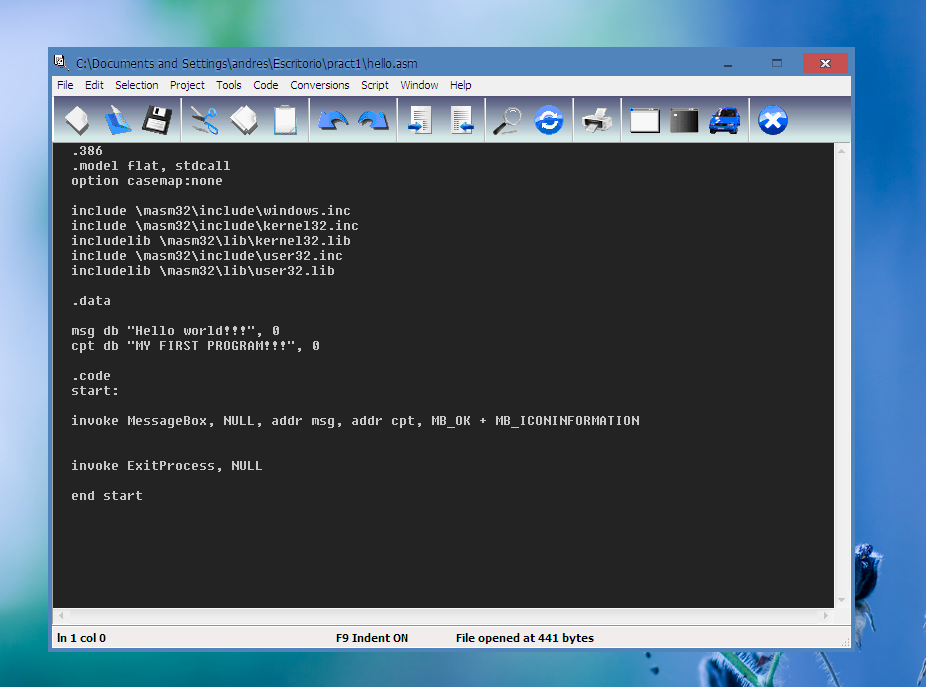
\includegraphics[width=\linewidth]{figs/fig1.png}
  \caption{Editor en MASM}
  \label{fig:1}
\end{figure}

\begin{figure}[ht]
  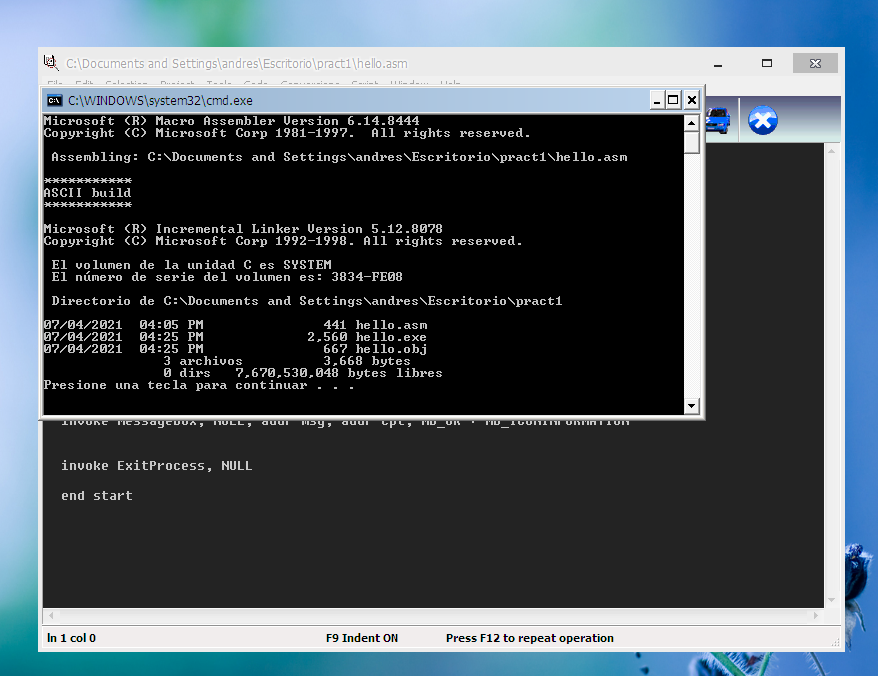
\includegraphics[width=\linewidth]{figs/fig2.png}
  \caption{ensamblaje en MASM}
  \label{fig:2}
\end{figure}

\begin{figure}[ht]
  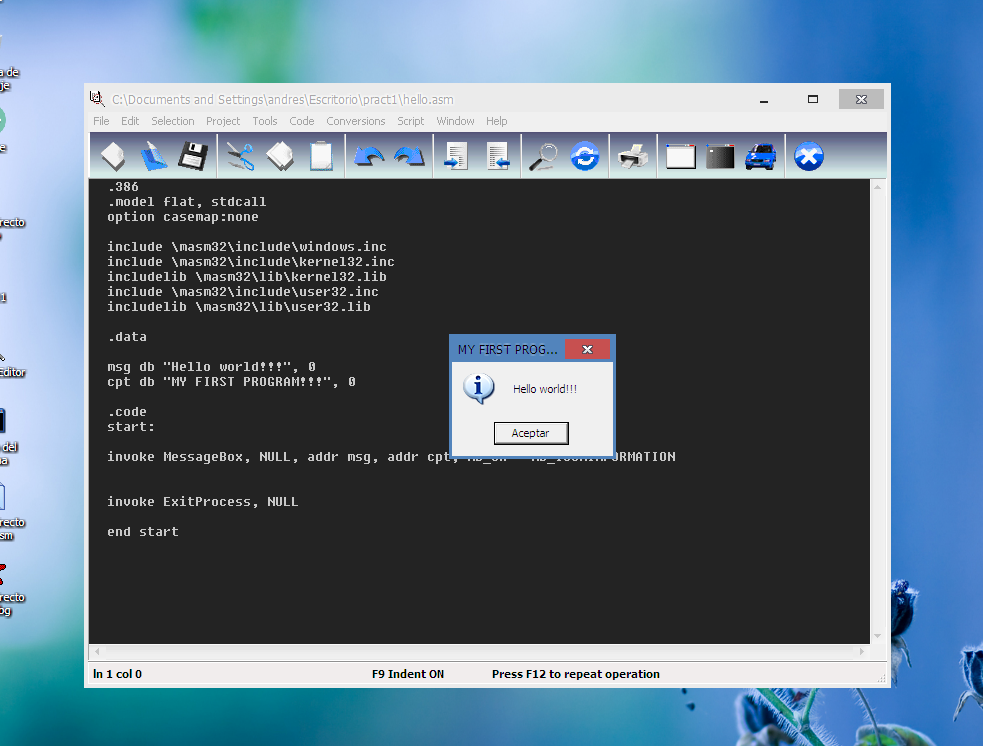
\includegraphics[width=\linewidth]{figs/fig3.png}
  \caption{Corriendo programa en MASM}
  \label{fig:3}
\end{figure}

